\section{Nonradial experiment: implementation and validation}
\label{sec:revision-experiments-details}

\subsection{Exact references and inverse-map cost}
We identify $\mathbb R^2$ with $\mathbb C$ and use a standard planar Gaussian label $Z$. Write $F_1(t,z)=e^{(1+i)at}z$ and $F_2(t,z)=b e^{(1+i)a\sqrt2t}z^2e^{-|z|^2}$, with $a=0.4$, $b=0.18$, and $F_t=F_1+F_2$. For the gauge parameter $\omega$, the exact trajectory from $F_0(z)$ is
\[
 X_t=F_t(e^{i(\omega-a)t}z).
\]
All tested gauge parameters therefore preserve the same continuous probability path. We evaluate the field in Cartesian coordinates: the algorithm receives $x$, recovers $z=F_t^{-1}(x)$ by contraction, and evaluates the velocity there. It does not evolve hidden labels instead of applying the stated numerical solver.

\begin{figure}[htbp]
\centering
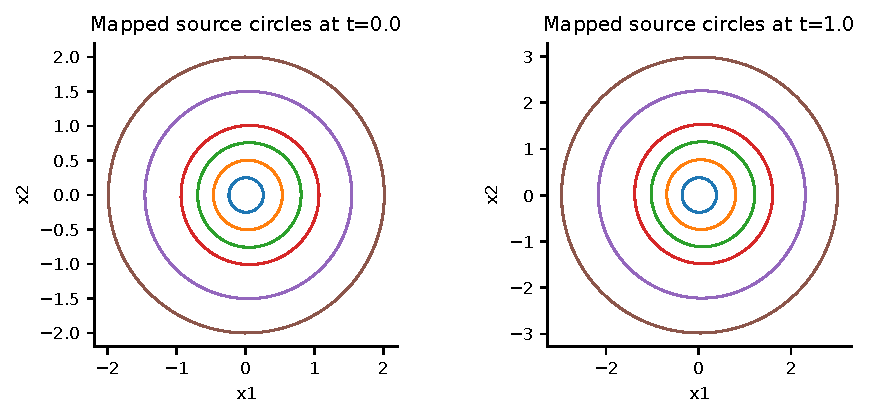
\includegraphics[width=0.85\linewidth]{../results/revision/harmonic_shape.pdf}
\caption{Images of concentric source circles under $F_0$ and $F_1$, showing the asymmetric deformation. These are mapped source contours, not claimed level sets of the target density.}
\end{figure}

Starting with $z_0=e^{-(1+i)at}x$, the inverse iteration is
\[
 z_{j+1}=e^{-(1+i)at}x-b e^{(1+i)a(\sqrt2-1)t}z_j^2e^{-|z_j|^2}.
\]
Its declared contraction factor is
$\rho_t=(4/e)b e^{a(\sqrt2-1)t}<0.313$.
We stop when $\rho_t\|z_{j+1}-z_j\|_\infty/(1-\rho_t)\le2\times10^{-14}$.
This is the exact-arithmetic contraction error bound evaluated in floating point, not a roundoff-inclusive enclosure. A refinement uses $2\times10^{-15}$. The main $N=512$ corrected-Euler run uses $8{,}319$ batch inverse iterations for $512$ field evaluations, about $16.25$ iterations per evaluation. Every solver stage, including every Heun and RK3 stage, pays this cost. No neural network, numerical score, numerical Jacobian, or Poisson solve is used in this example.

\subsection{An exact residual objective with an observable bad local minimum}
Set $n\in\{1,2\}$,
\[
 \zeta_n=a\sqrt n+i\{a\sqrt n+n(\omega-a)\},\qquad
 k_t(F_tz)=D F_t(z)Jz=\sum_{n=1}^2 inF_n(t,z).
\]
The acceleration along this gauge is $\sum_n\zeta_n^2F_n$.
The field $w_t=ck_t$ preserves $p_t$, so the following is an upper certificate for the weighted-gradient acceleration residual, not generally an equality with that projection norm:
\[
 R_t(\omega,c)^2
 =\|\mathbf a_\omega-ck_t\|_{L^2(p_t)}^2
 =\sum_{n=1}^2M_n(t)|\zeta_n^2-inc|^2,
\]
where
\[
 M_1(t)=2e^{2at},\qquad
 M_2(t)=\frac8{125}b^2e^{2a\sqrt2t}.
\]
The second identity follows from angular orthogonality and
$\mathbb E[|Z|^4e^{-2|Z|^2}]=8/125$.
Both masses increase, so $\sup_{0\le t\le1}R_t=R_1$ for fixed $(\omega,c)$.
Eliminating $c$ gives
\[
 c_*(\omega)=\frac{\sum_n nM_n(1)\operatorname{Im}(\zeta_n^2)}
                  {\sum_n n^2M_n(1)}.
\]
The remaining objective is a coercive quartic. The code enumerates all real roots of its cubic derivative, then compares objective values using the original sum of squares. Its three stationary points have $\omega$ approximately $-0.392394$, $0.000331763$, and $0.4$. Their residuals are approximately $0.0724104$, $0.3388934$, and floating-point zero. The first and third are local minima; the middle is a local maximum. Local least squares from $(\omega,c)=(-0.3,0)$ terminates at the inferior minimum. Starts $(0.07,0.03)$ and $(0.8,-0.2)$ reach the zero. The optimizer is therefore not treated as a global feasibility certificate; the finite stationary-point enumeration and the exact coefficient argument supply that distinction.

\begin{figure}[htbp]
\centering
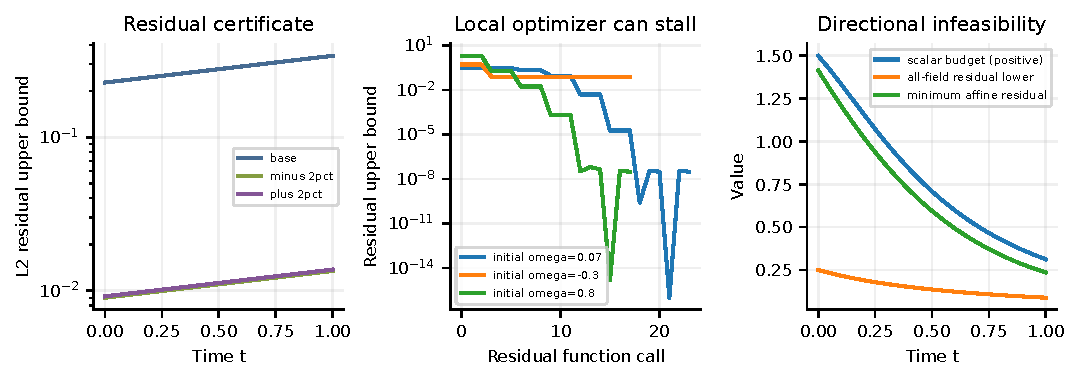
\includegraphics[width=\linewidth]{../results/revision/residual_discovery.pdf}
\caption{Left: exact formulas for residual upper certificates. The discovered solution is omitted from this logarithmic panel because its exact residual is zero. Center: local optimization from three initial values; the negative start stagnates at a positive residual. Right: the directional obstruction for a Gaussian path whose scalar energy budget is positive. The affine residual curve uses the global minimum of its even quartic objective.}
\end{figure}

\subsection{Distribution bounds and quadrature refinement}
For a numerical endpoint $\widehat X_N(Z)$, the lower bound is
\[
 \left|\sqrt{\mathbb E|\widehat X_N|^2}
       -\sqrt{M_1(T)+M_2(T)}\right|\le W_2(\widehat p_N,p_T).
\]
For corrected Euler, the upper bound uses the valid target coupling
$F_T(e^{-ia^2Th}Z)$, with $h=T/N$, as proved in Theorem~\ref{thm:harmonic-coupling}. For a perturbed $\omega$, we use
$F_T(e^{i\{(\omega-a)T-c_*(\omega)Th/2\}}Z)$.
Every such fixed rotation preserves the Gaussian source, so the pairing remains a valid upper bound even when no second-order guarantee is claimed. For base Euler, Heun, and RK3, the same-start coupling is used. We do not minimize these couplings or identify their RMS with full $W_2$.

The radial rule uses $s=|Z|^2/2\sim\operatorname{Exp}(1)$, with positive Gauss--Laguerre weights; the angular rule uses equally spaced points on $[0,2\pi)$. The main rule has $64\times64=4{,}096$ nodes. Refining to $96\times128=12{,}288$ nodes changes the $N=512$ corrected upper estimate by $7.8\times10^{-17}$ and the base upper estimate by less than $7\times10^{-15}$. The corrected lower estimate is unchanged at printed double precision. Tightening inverse tolerance by a factor ten changes the corrected upper estimate by less than $4\times10^{-18}$. A coarser $32\times32$ rule changes the corrected lower bound by about $3.1\times10^{-11}$; the fine rule is used throughout. This is a refinement study, not a rigorous quadrature error enclosure.

An independent DOP853 solve uses relative tolerance $2\times10^{-12}$ and absolute tolerance $2\times10^{-13}$ on five fixed labels, for the base, discovered, and $-2\%$-perturbed fields. Four observation times $1/4,1/2,3/4,1$ give a maximum discrepancy of $6.5\times10^{-12}$ from the analytic trajectories. Tests also compare acceleration with a second time difference of the exact nonlinear trajectory, so omission of the nonlinear-coordinate Hessian term would be detected.

\subsection{A path that passes the scalar budget but is infeasible}
Let $\Sigma_t=\operatorname{diag}(1+t,1+t+2t^2)$ and $p_t=\mathcal N(0,\Sigma_t)$. The gradient field is
$v_t=\frac12\dot\Sigma_t\Sigma_t^{-1}x$.
The scalar budget $\frac12(\operatorname{tr}\Sigma_t)''-\mathbb E|v_t|^2$ remains at least $0.3125$ over $[0,1]$. Nevertheless, $m_1(t)=\mathbb E X_1^2=1+t$ has zero second derivative and nonzero first derivative. Every admissible velocity satisfies
\[
 \mathbb E[u_1^2]\ge\frac1{4(1+t)},\qquad
 \mathbb E[X_1a_1]=-\mathbb E[u_1^2],\qquad
 \|P_{p_t}^{\nabla}\mathbf a_t\|_{L^2(p_t)}
 \ge\frac1{4(1+t)^{3/2}}.
\]
This is an all-field obstruction under the stated moment and integration-by-parts assumptions, not a failure of one optimizer.
As a diagnostic comparison, the code minimizes over all two-dimensional affine Gaussian gauges $A=v+\omega\Sigma^{1/2}J\Sigma^{-1/2}$. The acceleration's weighted-gradient projection is $Sx$, where
\[
 S\Sigma+\Sigma S=\ddot\Sigma-2A\Sigma A^\top,\qquad
 \varepsilon^2=\operatorname{tr}(S\Sigma S).
\]
This objective is an even quartic in $\omega$, so its global minimum follows from a quadratic minimization in $\omega^2\ge0$. The affine curve in the figure does not assert that every admissible non-affine field has the same minimum.

\subsection{A learned coefficient and a continuous-path error floor}
To separate learned-path error from integration error, define the restricted regression family
\[
 u_{\delta,\omega}(t,F_tz)
 =\partial_tF_tz+\delta D F_t(z)z+(\omega-a)D F_t(z)Jz.
\]
Its exact trajectory is $F_t(e^{\delta t}e^{i(\omega-a)t}z)$.
We observe $512$ independent pairs $(t,z)$, with $t$ uniform on $[0,1]$ and $z$ standard planar Gaussian, and noisy base velocities $v(t,F_tz)+\xi$, where the two coordinates of $\xi$ are independent $\mathcal N(0,0.08^2)$. Ordinary one-parameter least squares fits the coefficient of $D F_t(z)z$ around the specified base field. The true coefficient is zero; it is not supplied to the fit. Seeds $7,19,42$ give fitted coefficients approximately $-0.00060835$, $-0.00031947$, and $0.00253611$, respectively. Their known-noise standard errors are about $0.0020$. This experiment tests one identifiable coefficient with an exact model, not general neural velocity learning.

After adding the gauge $\omega=a$, the learned path is $p_t^\delta=(F_t\circ e^{\delta t})_\#\rho$. Its second moment is known exactly:
\[
 \mathbb E_{p_t^\delta}|X|^2
 =2e^{2at}s^2
  +b^2e^{2a\sqrt2t}\frac{8s^4}{(1+4s^2)^3},\qquad s=e^{\delta t}.
\]
We bound $W_2(p_T^\delta,p_T)$ below by the second-moment discrepancy and above by the common-label RMS between $F_T(e^{\delta T}Z)$ and $F_T(Z)$. These bounds give path-error intervals approximately
$[0.0012814,0.0012850]$,
$[0.0006730,0.0006749]$, and
$[0.0053504,0.0053654]$ for the three seeds.
At $N=512$, numerical-to-learned-path coupling upper bounds are between $8.9\times10^{-7}$ and $6.0\times10^{-6}$, while numerical-to-target error remains near these much larger path-error floors. The approximate fields are not claimed to satisfy exact acceleration preservation.

\begin{figure}[htbp]
\centering
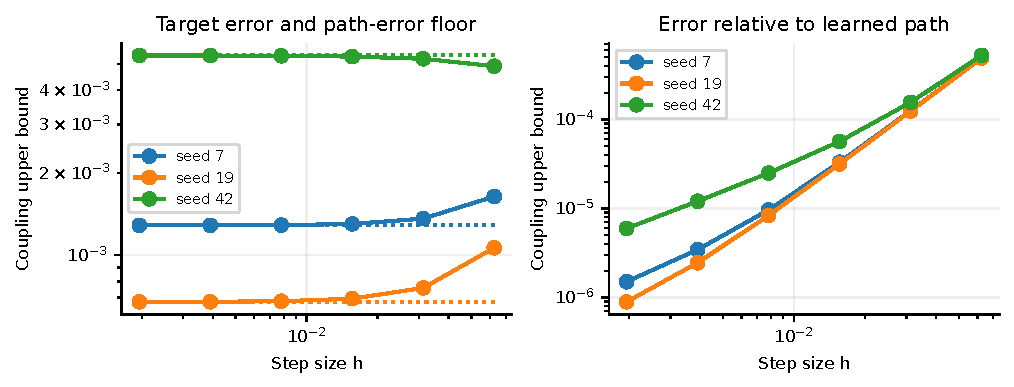
\includegraphics[width=\linewidth]{../results/revision/learned_path_floor.pdf}
\caption{Restricted learned-field experiment. Dotted lines are continuous-path coupling upper bounds. Integration refinement reduces error relative to the learned path but cannot remove error in the learned continuous distribution. Curves and floors are quadrature evaluations of valid upper couplings; they are not exact $W_2$ evaluations.}
\end{figure}

\subsection{Runtime, reproducibility, and limitations}
Equal-cost runs use budgets $48,96,192,384$ field evaluations; Euler uses $N$ steps, Heun $N/2$, and RK3 $N/3$. Each batch contains $4{,}096$ deterministic quadrature labels. Timings are the median of three repetitions, with minima and maxima retained in \texttt{equal\_cost.csv}. At $384$ evaluations, batch times are of the same order (a few tenths of a second) for all three methods. The correction search, including unsuccessful local searches, takes about $0.01$ seconds. The one-coefficient regression solve takes about $10^{-5}$ seconds after generating the data. These are CPU implementation measurements; they neither predict neural-network evaluation costs nor establish an end-to-end generation speedup. The observed Heun advantage is small, so we retain bounds and numerical refinement data rather than interpreting wall-clock differences of this size as significant. RK3's accuracy advantage is much larger.

\begin{figure}[htbp]
\centering
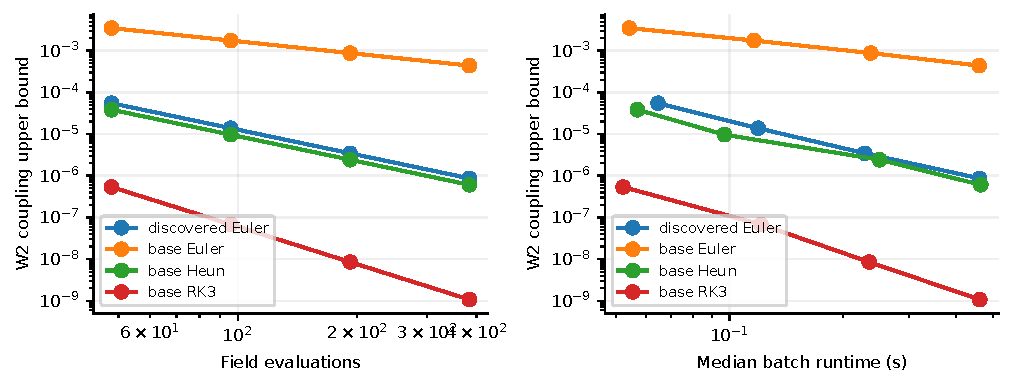
\includegraphics[width=\linewidth]{../results/revision/harmonic_cost.pdf}
\caption{Coupling upper bounds versus field-evaluation count and measured median batch runtime. The different methods use different couplings, so upper-bound curves alone do not order exact Wasserstein errors; Table~\ref{tab:revision-cost} also reports lower bounds.}
\end{figure}

The recorded environment is Linux x86\_64, Python 3.12.14, NumPy 2.3.5, and SciPy 1.17.0. The CPU reports Intel Xeon Platinum 8573C. We set \texttt{OMP\_NUM\_THREADS}, \texttt{OPENBLAS\_NUM\_THREADS}, and \texttt{MKL\_NUM\_THREADS} to one. The code does not claim a measured peak-memory advantage; it uses vectorized arrays of batch size $4{,}096$, and the exact small optimization eliminates any neural-training storage in this example.
Run
\begin{verbatim}
OMP_NUM_THREADS=1 OPENBLAS_NUM_THREADS=1 \
MKL_NUM_THREADS=1 python3 -B scripts/run_revision.py
python3 -B -m unittest discover -s tests -v
\end{verbatim}
from the repository root after installing the declared dependencies. The first command regenerates raw CSV files, the machine-readable summary, the table, and five figures under \texttt{results/revision/}. The original reproduction command regenerates the pre-existing Gaussian, nonlinear radial, and solver-comparison results separately. All $63$ original tests and $9$ new independent tests pass. The original reproduction regenerated $81$ baseline runs and $33$ nonlinear runs with $16{,}983$ and $24{,}600$ node comparisons, respectively; the original manuscript's rounded numerical macros agree exactly. No image-generation benchmark, high-dimensional learned model, or universal correction algorithm is claimed.
